
\section{\label{sec:RootsOfPolynomials}Akar Polinom}

\subsection{Meninjau Kembali Pembagian Sintetis\index{pembagian sintetis}\index{pembagian!sintetis}}

Anda mungkin masih ingat menggunakan teorema akar rasional dan pembagian
sintetis untuk menemukan akar polinom berderajat 3 atau lebih dalam
pelajaran aljabar. Prosesnya kurang lebih seperti berikut. Anda membuat
daftar akar yang mungkin berdasarkan teorema akar rasional. Anda memeriksa
setiap kandidat dengan pembagian sintetis hingga menemukan sebuah
akar atau kehabisan kandidat. Mungkin saja pelajaran Anda hanya membahas
proses itu sampai tahap tersebut, tetapi masih ada hal lain yang perlu
dibahas.

Misalkan kita mempunyai polinom $p(x)$ dan suatu bilangan $t$. Pembagian
sintetis memberikan koefisien-koefisien $q(x)$ sedemikian sehingga
$p(x)=q(x)\cdot(x-t)+p(t)$. Sebagai contoh, pembagian sintetis berikut

\begin{center}
\begin{tabular}{ccccc}
$\begin{gathered}t\\
\overbrace{\quad}
\end{gathered}
$ & \multicolumn{4}{c}{$\begin{gathered}p(x)\\
\overbrace{\qquad\qquad\qquad\qquad\qquad}
\end{gathered}
$}\tabularnewline
\multicolumn{1}{c|}{$-3$} & $-4$ & $2$ & $3$ & $-6$\tabularnewline
\cline{1-1}
 &  & $12$ & $-42$ & $117$\tabularnewline
\cline{2-5}
 & $-4$ & $14$ & \multicolumn{1}{c|}{$-39$} & \multicolumn{1}{c|}{$111$}\tabularnewline
\cline{5-5}
 & \multicolumn{3}{c}{$\begin{gathered}\underbrace{\qquad\qquad\qquad}\\
q(x)
\end{gathered}
$} & $\begin{gathered}\underbrace{\qquad\quad}\\
p(t)
\end{gathered}
$\tabularnewline
\end{tabular}
\par\end{center}

\noindent menunjukkan bahwa $p(x)=-4x^{3}+2x^{2}+3x-6=(-4x^{2}+14x-39)(x+3)+111$.
Menghitung nilai ekspresi $-4x^{3}+2x^{2}+3x-6$ ketika $x=-3$ hanya
memerlukan sedikit usaha, sedangkan menghitung nilai $(-4x^{2}+14x-39)(x+3)+111$
ketika $x=-3$ sama sekali tidak memerlukan usaha. Faktor $(x+3)$
bernilai nol, sehingga nilai $(-4x^{2}+14x-39)$ tidak menjadi soal.
Hasil kalinya nol dan $(-4x^{2}+14x-39)(x+3)+111$ bernilai $111$.
Oleh karena itu, $p(-3)=111$. Pembagian sintetis menyediakan cara
cepat untuk menghitung nilai sebuah polinom. Bilangan pada akhir pembagian
adalah nilai polinom pada bilangan yang digunakan untuk membentuk
pembagi.

Secara lebih umum, berikut adalah uraian pembagian $p(x)=a_{0}+a_{1}x+\cdots+a_{n}x^{n}$
oleh $x-t$ menggunakan pembagian sintetis:

\begin{center}
\begin{tabular}{cccccc}
\multicolumn{1}{c|}{$t$} & $a_{n}$ & $a_{n-1}$ & $a_{n-2}$ & $\cdots$ & $a_{0}$\tabularnewline
\cline{1-1}
 &  & $a_{n}t$ & $a_{n}(a_{n}t+a_{n-1})$ & $\cdots$ & $a_{n}(\cdots a_{n}(a_{n}(a_{n}t+a_{n-1})+a_{n-2})+\cdots+a_{1})$\tabularnewline
\cline{2-6}
 & $a_{n}$ & $a_{n}t+a_{n-1}$ & $a_{n}(a_{n}t+a_{n-1})+a_{n-2}$ & \multicolumn{1}{c|}{$\cdots$} & \multicolumn{1}{c|}{$p(t)$}\tabularnewline
\cline{6-6}
\end{tabular}
\par\end{center}

\noindent Dimulai dengan $t$ di sudut kiri atas, kita berakhir dengan
$p(t)$ di sudut kanan bawah. Kita tidak hanya menemukan sesuatu yang
menarik ketika bilangan di sudut kanan bawah bernilai nol. Setiap
pembagian sintetis menghasilkan sesuatu yang menarik! Bilangan di
sudut kanan bawah adalah $p(t)$, baik hasilnya nol maupun tidak.
Dan masih ada lagi.

Bilangan $a_{n}$, $a_{n}t+a_{n-1}$, $a_{n}(a_{n}t+a_{n-1})+a_{n-2}$,
dan seterusnya, yang muncul pada baris bawah pembagian sintetis, memberikan
koefisien hasil bagi, $q(x)$. Setiap pembagian sintetis memberikan
dekomposisi polinom menjadi hasil bagi dan sisa. Dengan demikian,
dari setiap pembagian sintetis kita memperoleh ekspresi ekuivalen
berbentuk $q(x)\cdot(x-t)+p(t)$. Masih ada lagi.

Mendiferensialkan persamaan $p(x)=q(x)\cdot(x-t)+p(t)$ terhadap $x$
menghasilkan
\[
p'(x)=q'(x)\cdot(x-t)+q(x).
\]
Oleh karena itu, $p'(t)=q'(t)\cdot(t-t)+q(t)=q(t)$. Jadi, bilangan-bilangan
pada baris bawah tidak hanya memberikan koefisien hasil bagi; bilangan-bilangan
tersebut sekaligus menjadi koefisien yang tepat untuk menghitung $p'(t)$.
Kembali ke contoh sebelumnya, jika kita ingin menghitung $p'(-3)$,
kita cukup melanjutkan pembagian sintetis seperti pada

\begin{center}
\begin{tabular}{ccccc}
\multicolumn{1}{c|}{$-3$} & $-4$ & $2$ & $3$ & $-6$\tabularnewline
\cline{1-1}
 &  & $12$ & $-42$ & $117$\tabularnewline
\cline{2-5}
\multicolumn{1}{c|}{$-3$} & $-4$ & $14$ & \multicolumn{1}{c|}{$-39$} & \multicolumn{1}{c|}{$111$}\tabularnewline
\cline{1-1}\cline{5-5}
 &  & $12$ & $-78$ & \tabularnewline
\cline{2-5}
 & $-4$ & \multicolumn{1}{c|}{$26$} & \multicolumn{1}{c|}{$-117$} & \tabularnewline
\cline{4-4}
\end{tabular}
\par\end{center}

\noindent dan kita memperoleh $p'(-3)=-117$. Prosedur menghitung
$p(t)$ dan $p'(t)$ melalui pembagian sintetis secara berturut-turut
dikenal sebagai metode Horner \index{metode Horner}\index{metode!Horner|see{metode Horner}}
dan sangat praktis digunakan dalam metode Newton. Jika kita mencoba
menemukan akar $p(x)=-4x^{3}+2x^{2}+3x-6$ dengan hampiran awal $x_{0}=-3$,
pada tahap ini kita akan memperoleh $x_{1}=x_{0}-\frac{p(x_{0})}{p'(x_{0})}=-3-\frac{111}{-117}\approx-2.05128$.
Namun, masih ada lagi.

\subsection{Menemukan Semua Akar Polinom}

\index{polinom!menemukan semua akar}Ketika kita menemukan sebuah
akar dari polinom $p(x)$, hasil pembagian sintetis, $p(x)=q(x)(x-t)+p(t)$,
menyederhana menjadi $p(x)=q(x)(x-t)$ karena $t$ merupakan akar,
yang berarti $p(t)=0$. Dalam kasus ini, kita memperoleh faktorisasi
$p(x)$. Akar-akar $p$ selebihnya tepat merupakan akar-akar $q$.
Jadi, setelah menemukan satu akar, kita telah mereduksi masalah pencarian
akar $p$ menjadi (a) mencatat akar yang telah ditemukan dan (b) mencari
akar polinom $q$, yang derajatnya satu lebih rendah daripada $p$.
Dengan cara ini, kita telah \index{deflasi} melakukan deflasi terhadap
masalah pencarian $n$ akar dari polinom berderajat $n$ yang dinyatakan
dengan $p$ menjadi pencarian $n-1$ akar dari polinom berderajat
$(n-1)$ yang dinyatakan dengan $q$. Melangkah lebih jauh, ketika
kita menemukan akar $q$, kita dapat menggunakan pembagian sintetis
untuk kembali mereduksi masalah. Kita (a) mencatat akar $q$ dan (b)
melanjutkan pencarian akar hasil baginya, yaitu polinom berderajat
$(n-2)$. Kita terus melakukannya, dengan mendeflasi masalah satu
derajat setiap kali menemukan akar, hingga masalah tersebut tereduksi
menjadi polinom berderajat $2$. Pada tahap ini, kita mempunyai polinom
kuadrat dan dapat menggunakan rumus kuadrat untuk menemukan dua akar
terakhir.

Sebagai contoh, $-1.18985$ merupakan (kira-kira) sebuah akar dari
$p(x)=-4x^{3}+2x^{2}+3x-6$. Pembagian sintetis $p(x)$ oleh $(x+1.18985)$
menghasilkan

\begin{center}
\begin{tabular}{ccccc}
\multicolumn{1}{c|}{$-1.18985$} & $-4$ & $2$ & $3$ & $-6$\tabularnewline
\cline{1-1}
 &  & $4.7594$ & $-8.04267$ & $6.00002$\tabularnewline
\cline{2-5}
 & $-4$ & $6.7594$ & \multicolumn{1}{c|}{$-5.04267$} & \multicolumn{1}{c|}{$0.00002$}\tabularnewline
\cline{5-5}
\end{tabular}
\par\end{center}

\noindent Nilai (hampir) nol di dalam kotak pada sudut kanan bawah
menunjukkan bahwa $-1.18985$ kira-kira merupakan sebuah akar. Tidak
terdapat sisa yang berarti ketika $-4x^{3}+2x^{2}+3x-6$ dibagi dengan
$x+1.18985$. Selain itu, bilangan $-4,6.7594,-5.04267$ pada baris
bawah memberikan koefisien $q(x)$. Dengan demikian, dari pembagian
ini kita memperoleh $-4x^{3}+2x^{2}+3x-6=\approx(-4x^{2}+6.7594x-5.04267)(x+118985)$.
Sekarang kita dapat menemukan dua akar lainnya dengan mencari akar
$q(x)=-4x^{2}+6.7594x-5.04267$. Dengan rumus kuadrat, akar-akarnya
adalah
\[
\frac{-6.7594\pm\sqrt{6.7594^{2}-4(-4)(-5.04267)}}{-8}\approx.84493\pm.73944i.
\]

Proses ini akan menghasilkan kesemua $n$ akar dari setiap polinom
berderajat $n$. Penting untuk dicatat bahwa sebagian akar tersebut
mungkin kompleks dan sebagian mungkin berulang. 

\begin{digression}{Teorema Dasar Aljabar}

\noindent Proses menemukan satu akar dari suatu polinom, melakukan
deflasi, lalu menemukan akar lainnya sangat selaras dengan teorema-teorema
matematika dalam aljabar. Teorema Dasar Aljabar\index{Teorema!Dasar Aljabar}
menyatakan bahwa setiap polinom berkoefisien kompleks dan berderajat
setidaknya satu memiliki sebuah akar kompleks. Jadi, pencarian akar
kita tidak sia-sia! Selanjutnya, kita dapat menuliskan polinom dalam
bentuk terfaktor dan melanjutkan proses. Teorema Dasar Aljabar menyatakan
bahwa polinom hasil deflasi itu juga memiliki sebuah akar. Jika kita
mencatat semua akar saat menemukannya, pada akhirnya kita menuliskan
polinom dalam bentuk
\begin{equation}
p(x)=a(x-r_{1})^{e_{1}}(x-r_{2})^{e_{2}}\cdots(x-r_{k})^{e_{k}},\label{eq:factoredPolynomial}
\end{equation}
Di sini, $a$ adalah konstanta tak nol, $r_{1},r_{2},\ldots,r_{k}$
adalah $k$ akar kompleks yang berbeda, dan $e_{1},e_{2},\ldots,e_{k}$
adalah apa yang disebut multiplisitas (bilangan bulat positif) dari
akar-akar tersebut. Dari bentuk ini kita melihat bahwa derajat polinom
sama dengan jumlah multiplisitas, $e_{1}+e_{2}+\cdots+e_{k}$. Inilah
yang dimaksud ketika kita mengatakan bahwa jumlah akar, jika multiplisitas
diperhitungkan, sama dengan derajat polinom. Jadi, ketika mencari
akar-akar polinom berderajat $n$, kita mengetahui bahwa kita mencari
$n$ akar, tetapi tidak harus $n$ akar yang berbeda. Sebagian dapat
berulang, dan pengulangannya diperhitungkan dalam multiplisitas. Untuk
merumuskan secara formal pernyataan dalam persamaan \ref{eq:factoredPolynomial},
kita memperoleh teorema berikut.
\begin{thm}
(Teorema Faktorisasi Fundamental)\index{Teorema!Faktorisasi Fundamental}
Jika $n\geq1$ dan $p$ adalah polinom berderajat $n$, maka 
\[
p(x)=a(x-r_{1})^{e_{1}}(x-r_{2})^{e_{2}}\cdots(x-r_{k})^{e_{k}}
\]
untuk suatu konstanta $a\neq0$, akar-akar $r_{1},r_{2},\ldots,r_{k}$,
dan eksponen bilangan bulat positif $e_{1},e_{2},\ldots,e_{k}$ yang
memenuhi
\[
\sum_{j=1}^{k}e_{j}=n.
\]
\end{thm}

\begin{proof}
Misalkan $n=1$, sehingga $p(x)$ berbentuk $ax+b$ dengan $a\neq0$.
Maka $p(x)=a(x-(-\frac{b}{a}))^{1}$ sehingga memenuhi bentuk yang
disyaratkan. Sekarang, misalkan semua polinom dengan suatu derajat
$n\geq1$ memenuhi bentuk yang disyaratkan, dan misalkan $p$ adalah
polinom berderajat $n+1$. Menurut Teorema Dasar Aljabar, $p$ mempunyai
sebuah akar. Namakan akar tersebut $\rho$. Maka $x-\rho$ adalah
faktor dari $p$, sehingga $p$ dapat ditulis sebagai $p(x)=(x-\rho)\cdot q(x)$
untuk suatu polinom $q$ berderajat $n$. Berdasarkan hipotesis induksi,
$q$ memenuhi bentuk yang disyaratkan, sehingga 
\[
p(x)=(x-\rho)\cdot a(x-r_{1})^{e_{1}}(x-r_{2})^{e_{2}}\cdots(x-r_{k})^{e_{k}}
\]
dengan $e_{1}+e_{2}+\cdots+e_{k}=n$. Jika $\rho$ berbeda dari $r_{1},r_{2},\ldots,r_{k}$,
maka $p$ berbentuk
\[
p(x)=a(x-r_{1})^{e_{1}}(x-r_{2})^{e_{2}}\cdots(x-r_{k})^{e_{k}}(x-\rho)^{1}.
\]
Jika $\rho$ sama dengan salah satu dari $r_{1},r_{2},\ldots,r_{k}$,
misalnya $r_{j}$, maka $p$ berbentuk 
\[
p(x)=a(x-r_{1})^{e_{1}}(x-r_{2})^{e_{2}}\cdots(x-r_{j})^{e_{j}+1}\cdots(x-r_{k})^{e_{k}}.
\]
Dalam kedua kasus, $p$ memenuhi bentuk yang disyaratkan, sehingga
pembuktian selesai.
\end{proof}
\end{digression}

\noindent Kode semu-semu untuk prosedur ini mungkin tampak seperti
berikut:

\noindent\begin{pseudocode}
\begin{description}
\item [{Asumsi:}] $p$ adalah polinom berderajat $n>2$.
\item [{Masukan:}] Polinom $p(x)$; toleransi $tol$; jumlah maksimum iterasi
$N$.
\item [{Langkah~1:}] Untuk $i=1$ hingga $n-2$, lakukan Langkah 2-5:

\begin{description}
\item [{Langkah~2:}] Temukan sebuah akar $x_{0}$ dari $p(x)$ {[}dengan
menggunakan $tol$, $N$, dan suatu metode pencarian akar{]};
\item [{Langkah~3:}] Jika terjadi galat saat mencari $x_{0}$, maka\\
$\qquad$kembalikan ``Metode gagal. Akar polinom berderajat $n-i+1$
tidak ditemukan.'';
\item [{Langkah~4:}] Faktorkan $p(x)$ sebagai $q(x)\cdot(x-x_{0})$;
\item [{Langkah~5:}] Tetapkan $x_{i}=x_{0}$; $p(x)=q(x)$;
\end{description}
\item [{Keluaran:}] Akar hampiran.
\end{description}
\end{pseudocode}

Untuk menyempurnakan kode semu-semu menjadi kode semu, kita akan menggunakan
metode Newton, dengan bantuan metode Horner, pada Langkah 2. Kelemahan
metode Newton yang lazim, yakni syarat bahwa turunannya harus diketahui
dan dihitung, hanyalah sedikit merepotkan ketika metode Horner digunakan.
Namun, bagaimana kita merepresentasikan polinom dalam program komputer
agar dapat melaksanakan Langkah 4 dan 5? Dengan cara yang sama seperti
ketika kita mengimplementasikan kode untuk menjalankan metode Horner.
Kode semu untuk metode Horner, dengan sebuah larik:\index{metode Horner!kode semu}

\noindent\begin{pseudocode}
\begin{description}
\item [{Asumsi:}] $p$ adalah polinom berderajat $n\geq1$.
\item [{Masukan:}] larik $[c]$ yang memuat koefisien $p(x)=c_{1}+c_{2}x+c_{3}x^{2}+\cdots+c_{n+1}x^{n}$;
$x_{0}$.
\item [{Langkah~1:}] Tetapkan $y=c_{n+1}$; $z=c_{n+1}$;
\item [{Langkah~2:}] Untuk $j=n,n-1,\ldots,2$, lakukan Langkah 3

\begin{description}
\item [{Langkah~3:}] Tetapkan $y=x_{0}y+c_{j}$; $z=x_{0}z+y$;
\end{description}
\item [{Langkah~4:}] Tetapkan $y=x_{0}y+c_{1}$;
\item [{Keluaran:}] $y=p(x_{0})$ dan $z=p'(x_{0})$.
\end{description}
\end{pseudocode}

Seperti dalam pembagian sintetis, variabel dengan berbagai pangkatnya
tidak perlu disimpan. Hanya koefisien yang diperlukan untuk mendefinisikan
sebuah polinom. Oleh karena itu, dalam program, polinom direpresentasikan
sebagai larik bilangan. Dengan menggabungkan kode semu-semu kita,
metode Newton, dan metode Horner menjadi satu program, kita memperoleh
metode untuk menemukan semua akar suatu polinom:

\noindent\begin{pseudocode}\label{pseudo:allroots}
\begin{description}
\item [{Asumsi:}] $p$ adalah polinom berderajat $n>2$ dan $c_{1}$, yaitu
koefisien konstanta dari $p$, tidak nol.
\item [{Masukan:}] larik $[c]$ yang memuat koefisien $p(x)=c_{1}+c_{2}x+c_{3}x^{2}+\cdots+c_{n+1}x^{n}$;
toleransi $tol$; jumlah iterasi maksimum $N$; nilai awal $x_{0}$.
\item [{Langkah~1:}] Tetapkan $m=n$;
\item [{Langkah~2:}] Untuk $i=1$ sampai $n-2$, lakukan Langkah 3-13:

\begin{description}
\item [{Langkah~3:}] Tetapkan $k=0$; tetapkan $x=x_{0}$;
\item [{Langkah~4:}] Selama $|x-x_{0}|>tol$ atau $k=0$, lakukan Langkah
5-12:

\begin{description}
\item [{Langkah~5:}] Jika $k=N$, maka kembalikan ``Metode gagal. Tidak
semua akar ditemukan.''
\item [{Langkah~6:}] Tetapkan $x_{0}=x$;
\item [{Langkah~7:}] Tetapkan $d_{m}=c_{m+1}$; $z=c_{m+1}$;
\item [{Langkah~8:}] Untuk $j=m,m-1,\ldots,2$, lakukan Langkah 9

\begin{description}
\item [{Langkah~9:}] Tetapkan $d_{j-1}=x_{0}d_{j}+c_{j}$; $z=x_{0}z+d_{j-1}$;
\end{description}
\item [{Langkah~10:}] Tetapkan $y=x_{0}d_{1}+c_{1}$; 
\item [{Langkah~11:}] Tetapkan $x=x_{0}-\frac{y}{z}$; 
\item [{Langkah~12:}] Tetapkan $k=k+1$;
\end{description}
\item [{Langkah~13:}] Tetapkan $r_{i}=x$; $[c]=[d]$; $m=m-1$;
\end{description}
\item [{Langkah~14:}] Tetapkan $D=\sqrt{c_{2}^{2}-4c_{1}c_{3}}$; $s_{1}=-c_{2}+D$;
$s_{2}=-c_{2}-D$;
\item [{Langkah~15:}] Jika bagian riil $c_{2}$ negatif, tetapkan $r_{n-1}=\frac{s_{1}}{2c_{3}}$
dan $r_{n}=\frac{2c_{1}}{s_{1}}$; jika tidak, tetapkan $r_{n-1}=\frac{s_{2}}{2c_{3}}$
dan $r_{n}=\frac{2c_{1}}{s_{2}}$;
\item [{Keluaran:}] Larik $[r_{1},r_{2},\ldots,r_{n}]$ yang berisi akar-akar
hampiran.
\end{description}
\end{pseudocode}

\noindent Langkah 4 sampai 12 menerapkan metode Newton untuk mencari
satu akar, dengan menggunakan metode Horner pada Langkah 7 sampai
10 untuk menghitung nilai polinom dan turunannya di $x_{0}$. Koefisien
$[d]$ dari hasil bagi dihitung dan disimpan dengan cermat agar mudah
dirujuk pada Langkah 13. Akar kuadrat yang dihitung pada Langkah 14
diasumsikan berada pada cabang utama akar kuadrat kompleks. Langkah
14 dan 15 menggunakan bentuk alternatif rumus kuadrat yang sebisa
mungkin menghindari pengurangan dua besaran yang nilainya hampir sama.

\noindent\begin{digression}{Rumus Kuadrat Alternatif}

\noindent\index{rumus kuadrat!alternatif}Jika akar-akar $p(x)=ax^{2}+bx+c$
bernilai kecil, pembilang dalam rumus kuadrat, $x=\frac{-b\pm\sqrt{b^{2}-4ac}}{2a}$,
tentu juga bernilai kecil. Dalam kasus ini, sebaiknya tanda dari $-b$
dan $\pm\sqrt{b^{2}-4ac}$ dibuat sama agar tidak terjadi pengurangan
antara besaran-besaran yang nilainya hampir sama. Memilih tanda suku
akar kuadrat dengan cara ini menghasilkan salah satu akar seakurat
mungkin, tetapi membiarkan akar lainnya belum ditentukan. Dengan mengalikan
pembilang dan penyebut dengan konjugat pembilang, diperoleh bentuk
alternatif rumus kuadrat:
\begin{eqnarray*}
\frac{-b\pm\sqrt{b^{2}-4ac}}{2a}\cdot\frac{-b\mp\sqrt{b^{2}-4ac}}{-b\mp\sqrt{b^{2}-4ac}} & = & \frac{b^{2}-(b^{2}-4ac)}{2a(-b\mp\sqrt{b^{2}-4ac})}\\
 & = & \frac{4ac}{2a(-b\mp\sqrt{b^{2}-4ac})}\\
 & = & \frac{2c}{-b\mp\sqrt{b^{2}-4ac}}.
\end{eqnarray*}
Jika kedua pilihan tanda dituliskan secara eksplisit, diperoleh
\[
\frac{-b+\sqrt{b^{2}-4ac}}{2a}=\frac{2c}{-b-\sqrt{b^{2}-4ac}}
\]
dan
\[
\frac{-b-\sqrt{b^{2}-4ac}}{2a}=\frac{2c}{-b+\sqrt{b^{2}-4ac}}.
\]

\noindent\end{digression}

\noindent Namun, tidak banyak yang dapat dilakukan pada tahap ini
jika nol ternyata merupakan akar ganda. Dalam keadaan ini, baik $c_{1}$
maupun $c_{2}$ akan bernilai nol atau hampir nol sehingga $s_{1}$
dan $s_{2}$ menjadi sangat kecil. Karena itulah kumpulan asumsi mencantumkan
syarat $c_{1}\neq0$. Syarat ini memastikan bahwa nol bukan akar dari
$p$. 

\subsection{Metode Newton dan polinom}

\index{metode Newton}Masih ada satu masalah lagi yang perlu ditangani
terkait penggunaan metode Newton untuk mencari akar polinom. Untuk
polinom berkoefisien riil, jika $x_{0}$ riil, maka $x_{1}$, $x_{2}$,
dan setiap iterasi berikutnya juga riil! Akar kompleks tidak akan
mungkin ditemukan. Hal ini bukan masalah jika polinom memiliki paling
banyak dua akar kompleks. Akar-akar riil akan ditemukan, dan polinom
kuadrat yang dihasilkan akan memuat kedua akar kompleks itu. Kedua
akar kompleks kemudian diperoleh dengan rumus kuadrat. Namun, secara
umum, kita tidak dapat mengandalkan bahwa suatu polinom memiliki paling
banyak dua akar kompleks. Metode kita harus dapat bekerja pada polinom
dengan sebanyak apa pun akar kompleks, termasuk ketika semua akarnya
kompleks.

Solusinya tidak sulit, dengan satu syarat. Secara matematis, metode
Newton dan metode Horner bekerja sama baiknya untuk bilangan kompleks
maupun bilangan riil. Selama bahasa pemrograman yang digunakan mampu
menangani bilangan kompleks, mulailah dengan hampiran awal kompleks
(bukan riil murni) $x_{0}$, dan akar kompleks akan ditemukan! Meskipun
demikian, mungkin saja semua akar riil ditemukan lebih dahulu sehingga
yang tersisa adalah polinom dengan lebih dari dua akar kompleks dan
tanpa akar riil. Di sinilah ketidakakuratan aritmetika titik-mengambang
justru membantu! Karena galat pembulatan, koefisien-koefisien maupun
nilai $x_{0}$ tidak akan benar-benar riil. Pada umumnya, akar-akar
kompleks akan ditemukan.

\subsection{Metode M�ller\label{subsec:mullers}}

Metode lain yang sangat cepat untuk mencari akar persamaan adalah
metode M�ller \index{metode M�ller}\index{metode!M�ller|see {metode M�ller}}.
Pada prinsipnya, metode ini sangat mirip dengan metode sekan. Dalam
metode sekan, dibuat dua hampiran awal $p_{0}$ dan $p_{1}$. Garis
sekan yang melalui titik $(p_{0},f(p_{0}))$ dan $(p_{1},f(p_{1}))$
digambar, dan perpotongannya dengan sumbu $x$ menghasilkan $p_{2}$.
Dalam metode M�ller diperlukan tiga hampiran awal $p_{0}$, $p_{1}$,
dan $p_{2}$. Parabola yang melalui titik $(p_{0},f(p_{0}))$, $(p_{1},f(p_{1}))$,
dan $(p_{2},f(p_{2}))$ digambar, dan perpotongannya dengan sumbu
$x$ menghasilkan $p_{3}$. Namun, ada dua masalah yang perlu diatasi.
Pertama, jika parabola yang digambar itu memotong sumbu $x$, parabola
tersebut memotongnya di dua titik. Kita perlu memilih salah satu nol
sebagai $p_{3}$. Kedua, mungkin saja parabola tersebut sama sekali
tidak memotong sumbu $x$. 

Masalah pemilihan akar mudah diselesaikan. Kita menganggap hampiran
$p_{2}$ lebih baik daripada yang lain, sehingga kita memilih akar
yang paling dekat dengan $p_{2}$. Sebenarnya, ini sekaligus menyelesaikan
``masalah'' kedua. Bahkan ketika parabola tidak memotong sumbu $x$,
parabola tersebut tetap memiliki nol. Nol-nol itu kompleks. Hal ini
tidak perlu dikhawatirkan. Kita cukup mengambil akar kompleks yang
paling dekat dengan $p_{2}$. Pendekatan ini memiliki keuntungan:
sekalipun semua koefisien $p(x)$ riil, $p_{0}$, $p_{1}$, dan $p_{2}$
semuanya riil, dan semua akar $p(x)$ kompleks, metode ini tetap dapat
menemukan sebuah akar kompleks.

Untuk mencari parabola yang melalui $(p_{0},f(p_{0}))$, $(p_{1},f(p_{1}))$,
dan $(p_{2},f(p_{2}))$, kita gunakan parabola $P(x)$ berbentuk
\[
P(x)=a(x-p_{2})^{2}+b(x-p_{2})+c.
\]
Dengan melakukan substitusi $x=p_{i}$ dan $P(x)=f(p_{i})$, diperoleh
tiga persamaan
\begin{eqnarray*}
f(p_{0}) & = & a(p_{0}-p_{2})^{2}+b(p_{0}-p_{2})+c\\
f(p_{1}) & = & a(p_{1}-p_{2})^{2}+b(p_{1}-p_{2})+c\\
f(p_{2}) & = & c
\end{eqnarray*}
Jadi, langsung diperoleh $c=f(p_{2})$, dan kita harus menyelesaikan
persamaan simultan
\begin{eqnarray*}
f(p_{0})-f(p_{2}) & = & a(p_{0}-p_{2})^{2}+b(p_{0}-p_{2})\\
f(p_{1})-f(p_{2}) & = & a(p_{1}-p_{2})^{2}+b(p_{1}-p_{2})
\end{eqnarray*}
untuk $a$ dan $b$. Solusinya adalah
\begin{eqnarray*}
b & = & \frac{(p_{0}-p_{2})^{2}(f(p_{1})-f(p_{2}))-(p_{1}-p_{2})^{2}(f(p_{0})-f(p_{2}))}{(p_{0}-p_{2})(p_{1}-p_{2})(p_{0}-p_{1})}\\
a & = & \frac{(p_{1}-p_{2})(f(p_{0})-f(p_{2}))-(p_{0}-p_{2})(f(p_{1})-f(p_{2}))}{(p_{0}-p_{2})(p_{1}-p_{2})(p_{0}-p_{1})}.
\end{eqnarray*}
Selanjutnya, dengan menyubstitusikan $a$, $b$, dan $c$ ke rumus
kuadrat, diperoleh akar $x=p_{2}-\frac{2}{b\pm\sqrt{b^{2}-4ac}}$.
Untuk memilih akar yang paling dekat dengan $p_{2}$, kita membandingkan
$|b+\sqrt{b^{2}-4ac}|$ dengan $|b-\sqrt{b^{2}-4ac}|$ dan menggunakan
yang nilainya lebih besar. Dengan demikian diperoleh nilai terkecil
untuk $|x-p_{2}|$, yaitu jarak akar dari $p_{2}$. 

Sebagai contoh, kita akan menggunakan metode M�ller dengan $p_{0}=1$,
$p_{1}=2$, dan $p_{2}=3$ untuk mencari sebuah akar dari $f(x)=x^{3}+1$.
Kita hitung
\begin{eqnarray*}
\delta_{0} & = & f(p_{0})-f(p_{2})=2-28=-26\\
\delta_{1} & = & f(p_{1})-f(p_{2})=9-28=-19\\
h_{0} & = & p_{0}-p_{2}=-2\\
h_{1} & = & p_{1}-p_{2}=-1\\
h_{2} & = & p_{0}-p_{1}=-1
\end{eqnarray*}
sehingga diperoleh $c=28$, $b=\frac{h_{0}^{2}\delta_{1}-h_{1}^{2}\delta_{0}}{h_{0}h_{1}h_{2}}=\frac{4(-19)-1(-26)}{-2}=25$,
dan $a=\frac{h_{1}\delta_{0}-h_{0}\delta_{1}}{h_{0}h_{1}h_{2}}=\frac{-1(-26)-(-2)(-19)}{-2}=6$.
Jika grafik $f(x)$ dan $P(x)=6x^{2}+25x+28$ diperhatikan dengan
saksama, tampak bahwa keduanya memang berpotongan di tiga titik (yakni
titik-titik yang disyaratkan), dan bahwa $P(x)$ tidak mempunyai akar
riil:

\begin{center}
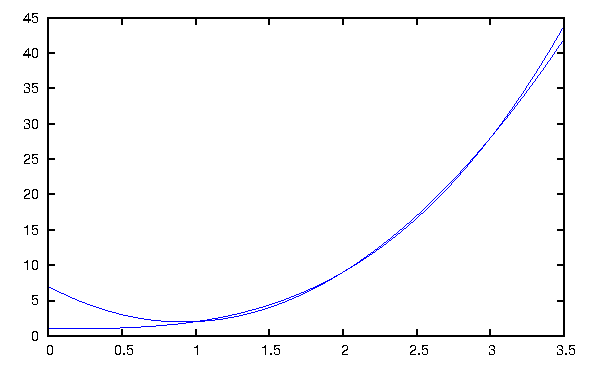
\includegraphics{figures/roots-polynomials02}.
\par\end{center}

\noindent$b\pm\sqrt{b^{2}-4ac}=25\pm\sqrt{625-672}=25\pm i\sqrt{47}$.
Karena $|25+i\sqrt{47}|=|25-i\sqrt{47}|$, akar mana pun dapat dipilih.
Dengan memilih $p_{3}=p_{2}-\frac{2c}{b-\sqrt{b^{2}-4ac}}$, diperoleh
$p_{3}=3-\frac{56}{25-i\sqrt{47}}=\frac{11}{12}-\frac{\sqrt{47}}{12}i$.
Jika proses ini dilanjutkan, diperoleh iterasi-iterasi $0.75238-0.75810i,\ 0.57069-0.84288i,\ldots,0.50000-0.86603i$,
yang konvergen ke $\frac{1}{2}-\frac{\sqrt{3}}{2}i$.

\begin{digression}{Orde Kekonvergenan}

\noindent\index{metode M�ller!orde kekonvergenan}Orde kekonvergenan
metode M�ller menuju akar sederhana (akar yang tidak berulang) adalah

\[
\left(\frac{\sqrt{11}}{3\sqrt{3}}+\frac{19}{27}\right)^{\frac{1}{3}}+\frac{4}{9\left(\frac{\sqrt{11}}{3\sqrt{3}}+\frac{19}{27}\right)^{\frac{1}{3}}}+\frac{1}{3}\approx1.839286755214161
\]
 dan menuju akar ganda adalah
\[
\left(\frac{\sqrt{139}}{24\sqrt{3}}+\frac{8}{27}\right)^{\frac{1}{3}}+\frac{7}{36\left(\frac{\sqrt{139}}{24\sqrt{3}}+\frac{8}{27}\right)^{\frac{1}{3}}}+\frac{1}{6}\approx1.233751928528259.
\]
 Metode Laguerre konvergen menuju akar sederhana dengan orde 3.
\begin{description}
\item [{Referensi}] \cite{muller,recipes}
\end{description}
\end{digression}

Tabel berikut merangkum keunggulan dan kelemahan relatif metode Newton,
metode sekan, dan metode M�ller.

\begin{center}
\begin{tabular}{c|ccc}
 & Newton & Sekan & M�ller\tabularnewline
\hline 
Nilai awal yang diperlukan & 1 & 2 & 3\tabularnewline
Perlu turunan? & Ya & Tidak & Tidak\tabularnewline
Orde Kekonvergenan\footnote{Orde yang dicantumkan berlaku untuk akar sederhana, bukan akar berulang.} & $2$ & $\approx1.618$ & $\approx1.839$\tabularnewline
Akar kompleks ditemukan secara otomatis? & Tidak & Tidak & Ya\tabularnewline
Lebih sederhana untuk polinom? & Ya & Tidak & Tidak\tabularnewline
\end{tabular}
\par\end{center}

\subsection{Konsep Utama}
\begin{description}
\item [{Pembagian~sintetis:}] \index{pembagian sintetis}Metode untuk
membagi polinom $p(x)$ dengan monomial $(x-x_{0})$ hanya dengan
menggunakan penjumlahan, perkalian, dan koefisien-koefisien $p$.
Proses ini identik dengan mengevaluasi polinom melalui penyarangan.
Pembagian sintetis sekadar menyediakan alat penataan agar penyarangan
dapat dilakukan dengan mudah menggunakan pensil dan kertas.
\item [{Metode~Horner:}] \index{metode Horner}Metode yang menghitung
nilai suatu polinom dan turunannya pada satu titik secara bersamaan
melalui pembagian sintetis.
\item [{Metode~M�ller:}] \index{metode M�ller}Metode pencarian akar yang
serupa dengan metode sekan, tetapi menggunakan parabola sebagai pengganti
garis sekan.
\item [{Deflasi:}] \index{deflasi}Metode untuk menyatakan suatu polinom
$p(x)$ sebagai hasil kali monomial $(x-x_{0})$ dan polinom $q(x)$
yang derajatnya satu lebih rendah daripada derajat polinom semula.
\end{description}
\startexercises 

\subsection{Latihan}
\begin{enumerate}
\item \label{exc:polynomials}\octave\ Tulislah sebuah fungsi Octave yang
menghitung akar-akar fungsi kuadrat dengan menggunakan bentuk alternatif
rumus kuadrat bila diperlukan. Baris pertama fungsi Anda harus berupa

\begin{center}
\texttt{function {[}r1,r2{]} = quadraticRoots(a,b,c)}
\par\end{center}

di mana \texttt{r1} dan \texttt{r2} merupakan akar-akar dari $p(x)=ax^{2}+bx+c$.
Dengan demikian, nilai \texttt{r1} dan \texttt{r2} dikembalikan oleh
fungsi dalam sebuah larik. Fungsi tersebut dipanggil seperti berikut:

\begin{center}
\texttt{{[}s,t{]}=quadraticRoots(1,2,3),}
\par\end{center}

yang menetapkan \texttt{s} sebagai nilai salah satu akar dan \texttt{t}
sebagai nilai akar lainnya. Uji kode Anda secara menyeluruh dengan
membandingkan keluaran fungsi Anda dengan hasil perhitungan manual
atau kalkulator.
\item \label{exc:polynomials-1}\octave\ Tulislah sebuah fungsi Octave
yang mengimplementasikan metode Horner. Baris pertama fungsi Anda
harus berupa 

\begin{center}
\texttt{function {[}p,pprime{]} = horner(x0,c)}
\par\end{center}

di mana \texttt{c} adalah larik yang memuat koefisien polinom, \texttt{x0}
adalah bilangan yang menjadi titik evaluasi polinom, \texttt{p} adalah
nilai polinom pada \texttt{x0}, dan \texttt{pprime} adalah nilai turunan
polinom pada \texttt{x0}. Dengan demikian, nilai \texttt{p} dan \texttt{pprime}
dikembalikan oleh fungsi dalam sebuah larik. Fungsi tersebut dipanggil
seperti berikut:

\begin{center}
\texttt{{[}y,yy{]}=horner(-2,{[}5,4,3,2,1{]}),}
\par\end{center}

yang menetapkan \texttt{y} sebagai nilai polinom dan \texttt{yy} sebagai
nilai turunannya. Uji kode Anda secara menyeluruh dengan membandingkan
keluaran fungsi Anda dengan hasil perhitungan manual atau kalkulator.
\item \label{exc:polynomials-2}\octave\ Tulislah sebuah fungsi Octave
yang mengimplementasikan metode Newton dengan metode Horner. Baris
pertama fungsi Anda harus berupa

\begin{center}
\texttt{function x = newtonhorner(c,x0,tol,N)}
\par\end{center}

di mana \texttt{c} adalah larik yang memuat koefisien polinom, \texttt{x0}
adalah nilai awal, \texttt{tol} adalah toleransi, dan \texttt{N} adalah
jumlah iterasi maksimum sebelum proses dihentikan. Kodenya harus serupa
dengan kode yang sebelumnya Anda tulis untuk mengimplementasikan metode
Newton, tetapi kode ini hanya berlaku untuk polinom. Di dalam fungsi
\texttt{newtonhorner}, JANGAN tuliskan kode metode Horner. Cukup panggil
fungsi \texttt{horner} yang Anda tulis pada soal \ref{exc:polynomials-1}.
Uji kode Anda secara menyeluruh dengan membandingkan keluaran fungsi
Anda dengan keluaran kode yang Anda tulis pada soal \ref{enu:newtonsMethodCode}
\vpageref{enu:newtonsMethodCode}.
\item \octave\ \label{exc:polynomials-12}Lengkapilah kode fungsi deflate
yang diawali di sini.\begin{verbatim}
% This function will deflate a polynomial
% given a root.
% INPUT: coefficients c of the polynomial;
%        a root r of the polynomial.
% OUTPUT: coefficients d of the deflated
%        polynomial.
function d = deflate(c,r)

end%function
\end{verbatim}
\item \octave\ Tulislah sebuah fungsi Octave yang mengimplementasikan metode
M�ller.
\item \label{exc:polynomials-3}Gunakan metode Horner/pembagian sintetis
untuk menentukan $g(2)$ dan $g'(2)$. Jangan gunakan komputer.

\begin{enumerate}
\item \label{exc:polynomials-6}$g(x)=3x^{3}+12x^{2}-13x-8$  \hasasolution 
\item \label{exc:polynomials-7}$g(x)=-7+8x-3x^{2}+5x^{3}-2x^{4}$ \hasananswer 
\end{enumerate}
\item \label{exc:polynomials-4}Gunakan metode Horner untuk menghitung $g(-2)$
dan $g'(-2)$ dengan $g(x)=4x^{4}-5x^{3}+6x-7$. Jangan gunakan komputer.
\item \label{exc:polynomials-10}Gunakan hasil pekerjaan Anda pada soal
\ref{exc:polynomials-3} untuk membantu melakukan dua iterasi metode
Newton dengan pensil, kertas, kalkulator, dan metode Horner/pembagian
sintetis. Gunakan nilai awal $x_{0}=2$. \haspartwithsolution  \haspartwithanswer 
\item Gunakan hasil pekerjaan Anda pada soal \ref{exc:polynomials-4} untuk
membantu melakukan dua iterasi metode Newton dengan pensil, kertas,
kalkulator, dan metode Horner/pembagian sintetis. Gunakan nilai awal
$x_{0}=-2$.
\item Hitung $x_{2}$ dari metode Newton secara manual (dengan menggunakan
metode Horner/pembagian sintetis) untuk $f(x)=x^{3}+4x-8$ dengan
nilai awal $x_{0}=0$.
\item Tentukan $x_{2}$ dari metode Newton secara manual (dengan menggunakan
metode Horner/pembagian sintetis) untuk $f(x)=x^{4}-2x^{3}-4x^{2}+4x+4$
dengan nilai awal $x_{0}=2$.
\item Dengan bantuan metode Horner dan tanpa menggunakan kalkulator, tentukan
iterasi pertama metode Newton untuk fungsi $f(x)=2x^{3}-10x+1$ dengan
nilai awal $x_{0}=2$.
\item Secara manual, tunjukkan dua iterasi metode Newton (dengan menggunakan
metode Horner/pembagian sintetis) yang diterapkan pada $f(x)=5x^{3}-2x^{2}+7x-3$
dengan $p_{0}=1$.
\item \label{findall}Carilah semua akar polinom dengan langkah-langkah
berikut. Gunakan metode Newton dengan toleransi $10^{-5}$ untuk menghampiri
salah satu akar polinom tersebut. Anda boleh menggunakan fungsi \texttt{newtonhorner}
yang Anda buat pada soal \ref{exc:polynomials-2}. Kemudian, gunakan
pembagian sintetis untuk melakukan deflasi pada polinom tersebut sehingga
derajatnya berkurang satu. Jangan gunakan komputer untuk deflasi.
Selanjutnya, gunakan metode Newton dengan toleransi $10^{-5}$ untuk
menghampiri salah satu akar polinom hasil deflasi. Kemudian, gunakan
kembali pembagian sintetis untuk melakukan deflasi pada polinom hasil
deflasi tersebut sehingga derajatnya berkurang satu lagi. Ulangi hingga
polinom hasil deflasi berderajat dua. Setelah itu, gunakan rumus kuadrat
(atau rumus kuadrat alternatif) untuk mencari dua akar terakhir.

\begin{enumerate}
\item \label{exc:polynomials-5}$g(x)=x^{4}+6x^{3}\text{\textminus}59x^{2}+144x\text{\textminus}144$ \hasasolution 
\item \label{exc:polynomials-14}$g(x)=-280+909x-154x^{2}-178x^{3}+54x^{4}+9x^{5}$ \hasananswer 
\end{enumerate}
\item Carilah semua akar polinom dengan langkah-langkah berikut. Gunakan
metode Newton dengan toleransi $10^{-5}$ untuk menghampiri salah
satu akar polinom tersebut. Anda boleh menggunakan fungsi \texttt{newtonhorner}
yang Anda buat pada soal \ref{exc:polynomials-2}. Kemudian, gunakan
pembagian sintetis untuk melakukan deflasi pada polinom tersebut sehingga
derajatnya berkurang satu. Anda boleh menggunakan fungsi \texttt{deflate}
yang Anda buat pada soal \ref{exc:polynomials-12} untuk proses deflasi
tersebut. Selanjutnya, gunakan metode Newton dengan toleransi $10^{-5}$
untuk menghampiri salah satu akar polinom hasil deflasi. Kemudian,
gunakan kembali pembagian sintetis untuk melakukan deflasi pada polinom
hasil deflasi tersebut sehingga derajatnya berkurang satu lagi. Ulangi
hingga polinom hasil deflasi berderajat dua. Setelah itu, gunakan
rumus kuadrat untuk mencari dua akar terakhir. Anda boleh menggunakan
fungsi \texttt{quadraticRoots} yang Anda buat pada soal \ref{exc:polynomials}
untuk menyelesaikan polinom kuadrat tersebut.

\begin{enumerate}
\item \label{exc:polynomials-16}$g(x)=x^{4}-2x^{3}-12x^{2}+16x-40$ \hasasolution 
\item \label{exc:polynomials-17}$g(x)=56-152x+140x^{2}-17x^{3}-48x^{4}+9x^{5}$ \hasananswer 
\end{enumerate}
\item \label{exc:polynomials-18}Untuk setiap akar yang Anda temukan pada
soal \ref{findall}, selain akar pertama, gunakan akar tersebut sebagai
hampiran awal dalam metode Newton dengan toleransi $10^{-5}$ untuk
melihat apakah Anda dapat memperbaiki hampiran akar tersebut. Apakah
hasilnya berubah? \haspartwithsolution  \haspartwithanswer 
\item $f(x)=x^{3}-1.255x^{2}-.9838x+1.2712$ memiliki akar di $x=1.12$.

\begin{enumerate}
\item Gunakan metode Newton dengan hampiran awal $x_{0}=1.13$ untuk mencoba
menemukan akar ini. Jelaskan apa yang terjadi.
\item Carilah semua akar $f(x)$.
\end{enumerate}
\item Sekitar 800 tahun lalu, John dari Palermo menantang para matematikawan
untuk mencari solusi persamaan $x^{3}+2x^{2}+10x=20$. Pada tahun
1224, Fibonacci menjawab tantangan tersebut di hadapan Kaisar Frederick
II. Ia menghampiri satu-satunya akar riil dengan teknik geometris
Omar Khayyam (1048-1131), hingga memperoleh taksiran
\[
\begin{gathered}1+22\left(\frac{1}{60}\right)+7\left(\frac{1}{60}\right)^{2}+42\left(\frac{1}{60}\right)^{3}+\\
\qquad\qquad33\left(\frac{1}{60}\right)^{4}+4\left(\frac{1}{60}\right)^{5}+40\left(\frac{1}{60}\right)^{6}.
\end{gathered}
\]
Seberapa akuratkah hampirannya?

\begin{description}
\item [{Referensi}] \cite[hlm. 96, soal 10]{burdenfaires}
\end{description}
\item \octave\ Hitung nilai polinom untuk nilai $x$ yang diberikan dengan
dua cara berbeda. (i) Gunakan fungsi \texttt{horner} yang Anda buat
pada soal \ref{exc:polynomials-1}; dan (ii) gunakan fungsi anonim.
Kemudian, (iii) bandingkan kedua hasil tersebut menggunakan operator
\texttt{==} pada Octave.

\begin{enumerate}
\item \label{exc:polynomials-8}$p(x)=x^{4}-2x^{3}-12x^{2}+16x-40$ pada
$x=\sqrt{3}$ \hasasolution 
\item \label{exc:polynomials-9}$q(x)=56-152x+140x^{2}-17x^{3}-48x^{4}+9x^{5}$
pada $x=\pi/2$ \hasananswer 
\item \label{exc:polynomials-11}$r(x)=x^{6}+11x^{4}-34x^{3}-130x^{2}-275x+819$
pada $\frac{1-\sqrt{5}}{2}$ \hasananswer 
\item $s(x)=5x^{10}+3x^{8}-46x^{6}-102x^{4}+365x^{2}+1287$ pada $\frac{1}{e}$
\end{enumerate}
\item \label{exc:polynomials-13}Tulislah fungsi Octave yang menggunakan
fungsi-fungsi Anda dari soal \ref{exc:polynomials}, \ref{exc:polynomials-2},
dan \ref{exc:polynomials-12} untuk mencari semua akar suatu polinom.
Uji fungsi Anda secara menyeluruh pada polinom-polinom dengan berbagai
derajat yang akar-akarnya telah Anda ketahui. Anda boleh mendasarkan
fungsi Anda pada kode semu \vpageref{pseudo:allroots}, tetapi kode
Anda seharusnya jauh lebih sederhana karena Anda cukup memanggil fungsi-fungsi
tersebut alih-alih menuliskan ulang kodenya. \hasananswer 
\item \label{exc:polynomials-15}Gunakan kode Anda dari soal \ref{exc:polynomials-13}
untuk mencari semua solusi persamaan berikut. \hasananswer 

\begin{enumerate}
\item $x^{5}+11x^{4}-34x^{3}-130x^{2}-275x+819=0$
\item $5x^{5}+3x^{4}-46x^{3}-102x^{2}+365x+1287=0$
\end{enumerate}
\item Carilah semua akar $g(x)=25x^{3}-105x^{2}+148x-174$.
\item Ingatlah bahwa metode sekan dan metode M�ller memiliki beberapa kemiripan.
Keduanya memerlukan beberapa hampiran awal. Keduanya melibatkan penentuan
nol suatu fungsi yang melalui titik-titik awal tersebut. Keduanya
konvergen secara superlinear menuju akar sederhana. Dan tentu saja,
keduanya merupakan metode pencarian akar. Mari kita ubah sedikit gagasan
ini sebagai berikut. Untuk mencari akar dari $g$, mulailah seperti
pada metode sekan dengan menggunakan dua hampiran, $x_{0}$ dan $x_{1}$.
Kemudian, alih-alih menggunakan nol dari garis yang melalui $(x_{0},g(x_{0}))$
dan $(x_{1},g(x_{1}))$, carilah fungsi berbentuk
\[
h(x)=ax^{3}+b
\]
yang melalui $(x_{0},g(x_{0}))$ dan $(x_{1},g(x_{1}))$. Misalkan
$x_{2}$ merupakan nol dari $h$. Kemudian, ulangi proses tersebut
dengan $x_{1}$ dan $x_{2}$ untuk memperoleh $x_{3}$, dan seterusnya.

\begin{enumerate}
\item Misalkan $g(x)=2\ln(1+x^{2})-x$, $x_{0}=5$, dan $x_{1}=6$. Tentukan
$x_{2}$ dengan menggunakan metode ini.
\item Carilah rumus untuk $x_{2}$ jika diberikan sebarang fungsi $g(x)$
dan sebarang kondisi awal $x_{0}$ dan $x_{1}$. Rumus tersebut harus
dinyatakan dalam $x_{0}$, $x_{1}$, $g(x_{0})$, dan $g(x_{1})$.
\item Carilah rumus umum untuk $x_{n}$ yang dinyatakan dalam $x_{n-2}$,
$x_{n-1}$, $g(x_{n-2})$, dan $g(x_{n-1})$.
\item \octave\ Tulislah fungsi Octave yang mengimplementasikan metode ini
dan menampilkan hasil setiap iterasi.
\item \octave\ Gunakan fungsi Octave Anda untuk menentukan apakah orde
kekonvergenan metode ini linear atau superlinear.
\end{enumerate}
\item Pilihlah fungsi yang akar-akarnya Anda ketahui secara eksak. Gunakan
metode M�ller untuk mencari salah satu akar tersebut. Gunakan tiga
iterasi berurutan untuk memperkirakan orde kekonvergenannya.
\item Galat dalam tiga iterasi berurutan metode M�ller ditampilkan dalam
tabel. Gunakan informasi ini untuk memperkirakan orde kekonvergenannya.

\begin{center}
\begin{tabular}{|c|c|}
\hline 
$n$ & $|x_{n}-x|$\tabularnewline
\hline 
\hline 
12 & $1.53627(10)^{-349}$\tabularnewline
\hline 
13 & $1.67365(10)^{-642}$\tabularnewline
\hline 
14 & $1.83922(10)^{-1181}$\tabularnewline
\hline 
\end{tabular}
\par\end{center}
\item \label{exc:polynomials-19}Grafik $f(x)$ ditampilkan. Carilah beberapa
himpunan nilai $p_{0}$, $p_{1}$, dan $p_{2}$ yang berbeda satu
sama lain, sehingga metode M\"uller

\begin{enumerate}
\item akan menghasilkan nilai kompleks untuk $p_{3}$.
\item akan menghasilkan akar di $x\approx4.4$.
\item akan menghasilkan akar di $x\approx2.8$.
\end{enumerate}
\begin{center}
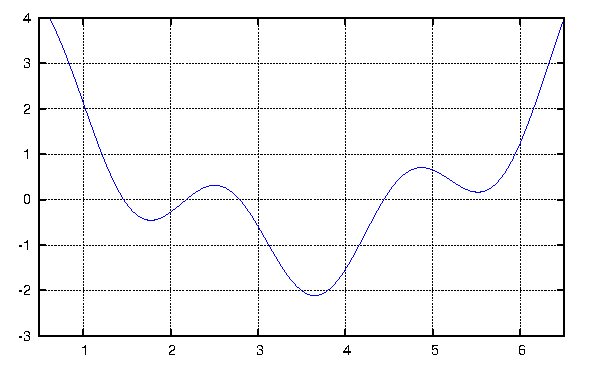
\includegraphics[scale=0.7]{figures/roots-polynomials01}
\par\end{center}
\item \octave\ Fungsi yang ditampilkan pada soal \ref{exc:polynomials-19}
adalah $f(x)=\frac{x^{2}-7x+10}{2}+\sin(3x)$. Gunakan informasi ini
untuk menguji dugaan-dugaan Anda pada soal \ref{exc:polynomials-19}.
\end{enumerate}
\finishexercises 
